%se debe compilar 2 veces para ver los cambios en el indice y otros sitios.

%tamaño de letra 12, tamaño carta, margen de un solo lado (sin oneside queda bonito pero no creo que les guste)
\documentclass[12pt,oneside, letterpaper]{book}

%documento en español<
\usepackage[spanish]{babel}

%para los acentos directos, se pueden usar así o as\'i
\usepackage[utf8]{inputenc}

%para agregar las imagenes
\usepackage{graphicx}
\graphicspath{ {images/} }

%Titulo del trabajo
\title{Lineamientos para Soluciones de Alta Disponibilidad en VoIP}

%autores
\author{Br. Sebastian Suarez \and
		Br.Dorjes Molina}
	
%fecha de entrega	(ojalá)
\date{Diciembre 2016}

\begin{document}
	
	%sin numero de pagina
	\pagenumbering{gobble}
	
	%página de titulo
	\maketitle
	\newpage
	


	%números de pagina en romano
	\pagenumbering{roman}
	\newpage
	
	%indice
	\addtocontents{toc}{~\hfill\textbf{P\'agina}\par}
	\setcounter{tocdepth}{5}
	\tableofcontents
	
	\newpage
	
	%indice de figuras y tablas
	\listoffigures
	
	\newpage
	\listoftables
	
	%glosario de terminos (ubicar y llenar)
	\chapter*{Glosario de terminos}

	\newpage
	
	%números de pagina en números normales
	\pagenumbering{arabic}

	%primera parte
%	\part{Marco Teórico}
%	\section{Introducci\'on}
%	\section{Telefon\'ia Tradicional}
%	\section{Modelo de capas}
%	\subsection{OSI}
%	\subsection{TCP/IP}
	\chapter{Voz sobre Protocolo de Internet}
		
	\section{VoIP}
	
	La voz sobre protocolo de internet, VoIP por sus siglas en 
	inglés “Voice over Internet Protocol”, es el término usado 
	para referirse a la tecnología que se aprovecha de la 
	infraestructura de transmisión de datos existente para 
	transportar la voz, previamente encapsulada dentro de paquetes 
	de datos, utilizando el protocolo de internet (IP) sobre 
	redes públicas o privadas. En términos más simples, VoIP 
	es un servicio telefónico a través de la red de datos, 
	que se encarga de digitalizar, comprimir y encapsular 
	señales de audio analógicas para que sean enviadas y recibidas 
	a través de redes compatibles con el protocolo IP.
	
	%insertar imagenes, "h" es para insertarla flotante 
	%en la posicion exacta donde está, debajo del texto superior.
	\begin{figure}[h]
		
		%nombre de la imagen, sin extencion. "width=\textwidth" ancho igual al texto
		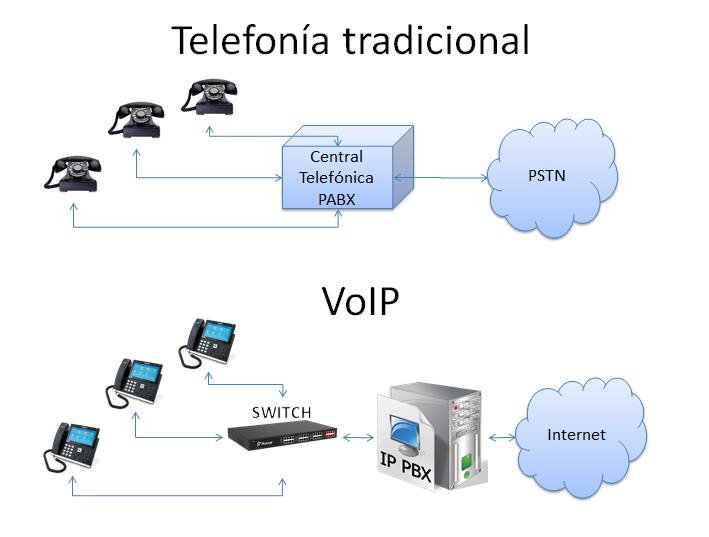
\includegraphics[width=\textwidth]{tradicionalVSvoip}
		
		%titulo de la imagen, salen debajo de la imagen y en el indice de imagenes.
		\caption{Telefonía tradicional versus VoIP}
		
		%centrado, por si las moscas
		\centering
		
		%para referencias
		\label{fig:ttvsv}
	\end{figure}

	Es muy importante diferenciar entre voz sobre IP (VoIP) y telefonía sobre IP 
	(ToIP) [Figura \ref{fig:ttvsv}]. Algunos autores \cite{switching} indican que 
	en forma general tanto VoIP como ToIP son términos intercambiables. Otros 
	\cite{voiptoip} definen a VoIP como el conjunto de normas, dispositivos, 
	protocolos que intervienen en la transmisión de voz sobre el protocolo IP, 
	conformando de esa forma una tecnología. Mientras que ToIP es el servicio 
	telefónico disponible al público basado en la tecnología VoIP, así como el conjunto de nuevas 
	funcionalidades que se ofrecen gracias al uso de la tecnología VoIP integrando 
	los servicios de datos y de voz, tanto analógica como digital. 
	
	En el presente documento se hará uso del término VoIP como la tecnología, 
	incluyendo los nuevos servicios integrados que se ofrecen gracias a esta 
	y el termino ToIP como el acto de simular aplicaciones de telefonía 
	tradicional a través del uso de VoIP.
	
	\begin{figure}[h]
		
		%nombre de la imagen, sin extencion. "width=\textwidth" ancho igual al texto
		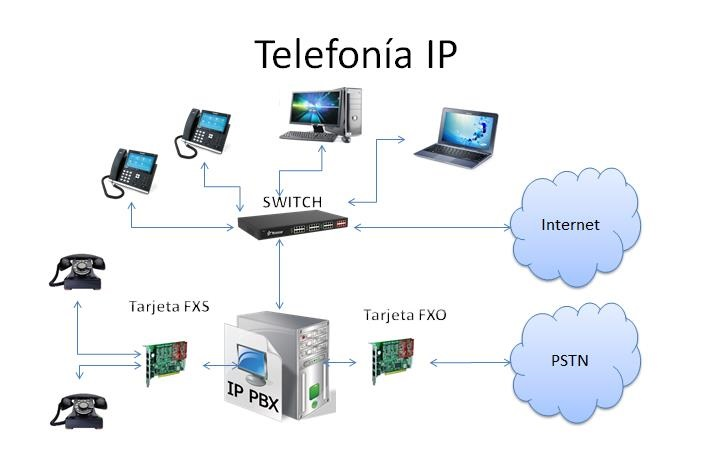
\includegraphics[width=\textwidth]{toip}
		
		%titulo de la imagen, salen debajo de la imagen y en el indice de imagenes.
		\caption{Esquema básico de Telefonía IP}
		
		%centrado, por si las moscas
		\centering
		
		%para referencias
		\label{fig:toip}
	\end{figure}

	
	
	


	\section{Antecedentes}
	
	En el pasado, la tecnología VoIP era de baja calidad, puesto que los algoritmos 
	de compresión no eran sofisticados y la capacidad de transmisión de los medios 
	digitales era bastante baja, sin embargo, la tecnología ha avanzado lo suficiente 
	como para incluso mostrarse como un competidor robusto contra la telefonía tradicional.
	 
	Aunque la tecnología VoIP no es precisamente reciente, el auge actual en las tecnologías 
	de comunicación, así como el aumento de la velocidad de los enlaces digitales y el alto 
	costo de las tarifas telefónicas proyectando el crecimiento de la tecnología VoIP en los últimos años.
	
	VoIP inicia casi inmediatamente después de la liberación de la Internet (1994) para uso público. 
	En 1995 un grupo de jóvenes israelíes que pretendían transmitir voz de un computador a 
	otro crearon el primer “softphone” (programa de computador que emula el comportamiento 
	de un teléfono) llamado Internet Phone Software o Vocaltech phone, desafortunadamente 
	la tecnología en aquel momento limitaba mucho la calidad del servicio, por lo que no 
	tuvo mucho éxito. Luego, en 1997 aparecen las primeras PBX (Private Branch Exchange), 
	prolifera el uso de protocolo H323 para transmisión de audio y video, aunque a baja 
	calidad por el ancho de banda costoso y de baja capacidad. Para el año 2000 ya Asterisk 
	y el protocolo SIP habían ingresado en el mercado VoIP, aunque las empresas todavía no 
	confían en Linux por lo que se mantienen usando PBX privativas y H323. 
	
	En el año 2003 Skype entra en el mercado, Asterisk introduce el protocolo IAX y el 
	costo de los teléfonos IP se reduce un 50\%. En los próximos años surge la Astricon, 
	una convención internacional de usuarios de Asterisk, se desarrollan mejoras en Skype 
	y en el protocolo IAX (surge IAX2), se reducen más los precios de los terminales VoIP, 
	Google incursiona en la tecnología al lanzar GoogleTalk. Para 2006 Skype logra alcanzar 
	50 millones de usuarios. En los siguientes años surgieron otros servicios como Google 
	Voice en 2009 y Viber en 2010. La era móvil ha impulsado la masificación de VoIP al 
	aprovechar una de sus principales características, la movilidad, para el 2012 las 
	aplicaciones móviles como Line, Yuliop y Whatsapp incluyen llamadas gratuitas entre 
	usuarios a través de internet. 
	
	En los últimos años la tecnología VoIP ha tomado gran auge gracias a las mejoras 
	en la infraestructura de la red y al interés por reducir cada vez más los costos 
	asociados a las telecomunicaciones, principalmente en empresas pequeñas o 
	emprendimientos.
	\section{Características}

	La telefonía IP puede realizar las mismas funciones de la telefonía tradicional 
	e incluso ofrece funciones adicionales como: Monitoreo de llamadas, Recuperación 
	de llamadas, Transferencia de llamadas, Grabación de llamadas, Identificación de 
	usuarios, Videoconferencias, Mensajería SMS, Música en espera, Llamadas en espera, 
	Recepción y transmisión de fax, Llamadas de emergencia, Llamadas automáticas, 
	entre otras.
	
	Las ventajas de la telefonía IP sobre la telefonía tradicional no se limitan 
	solo a funciones adicionales, sino que también presentan un conjunto de 
	bonificaciones entre las que se destaca: 
	
	\begin{itemize}
		\item Reducción de costos de instalación: VoIP requiere de una infraestructura 
		similar a la red de datos, por tanto, se puede integrar en la misma red o 
		aprovechar parte de la red existente. 
		\item Reducción de costos de mantenimiento: Como el equipo de VoIP es similar 
		al de red de computadoras ya instalada, el equipo técnico ya está familiarizado 
		con problemas habituales de conectividad, por lo que no se requiere de contratar 
		a terceros para solucionar problemas.
		\item Escalabilidad: Aumentar la capacidad de la red es micho más sencillo 
		comparado con telefonía tradicional y las inversiones monetarias son incluso
		 menores.
		\item Seguridad: Aunque la seguridad  en VoIP depende principalmente de la 
		seguridad de la red de datos, VoIP posee funcionalidades adicionales como 
		cifrado de la voz digitalizada o autenticación, autorización y protección 
		de los datos que viajan en su red.
		\item Compatibilidad:  Los estándares de la industria facilitan la compatibilidad
		 entre dispositivos o programas de distintos fabricantes, lo que facilita el 
		 acceso a la tecnología.
		\item Integración de servicios: Si bien VoIP sirve como plataforma para una central 
		telefónica, la gran variedad de funcionalidades adicionales que posee aumentan su 
		potencial. Integrar voz, video y datos en una misma red es uno de los pilares
		 de VoIP.
		\item Calidad de servicio: Permite asignar prioridad a los datagramas que viajan 
		por el medio lo que permite garantizar la transmisión de la conversación bajo un 
		umbral de considerable calidad.
		\item Movilidad: Siempre que se tenga una conexión a Internet, su servicio de 
		VoIP estará disponible en cualquier parte del mundo, podrá enviar y recibir 
		llamadas desde el mismo número de teléfono o extensión. 
	\end{itemize}
		
\section{VoIP frente a la telefonía tradicional}
	
	Las capacidades de la telefonía tradicional están directamente relacionadas con la cantidad de conexiones físicas de la red, ya que cada llamada debe establecerse a través de un circuito. Por tanto, muchas de las limitaciones de la telefonía tradicional surgen principalmente de la tecnología de conmutación de circuitos 
	usada por esta.
	
	En telefonía tradicional, las compañías tardan más tiempo en implementar nuevas características (como llamadas en espera o llamadas en 3 vías) e incluso pueden no ser implementadas en toda la red al mismo tiempo. La fidelidad del sonido está limitada al ancho de banda disponible entre el emisor y el destino de la 
	llamada, y el número máximo de llamadas entre dos locaciones está limitado a la disponibilidad de circuitos de voz disponibles entre ellas. Aumentar la capacidad del sistema implica aumentar la capacidad de circuitos y esto se traduce en una inversión monetaria. 
	 
	Las compañías de telefonía tradicional han logrado hacer muchos avances en identificar y resolver problemas relacionados con capacidad y costo. La implementación de líneas T1 o T3 han reducido los costos de la telefonía, la introducción de características como rutas de menor costo (LCR, least cost routing) a las PBX han reducido los costos de las llamadas de larga distancia.
	 
	En su momento, las características de la telefonía tradicional fueron consideradas como ventajas competitivas. Estas tecnologías, al ser  implementadas por una empresa, se volvían parte del costo de “hacer negocios”. Pero, la llegada de la Internet trajo consigo innovadores en busca de nuevas soluciones y las diferencias en la ingeniería y filosofía de estas tecnologías parecían indicar que el Internet era superior a las redes de voz tradicionales en muchos sentidos.
	 
	En la Internet, los protocolos de comunicación son mejorados constantemente por lo que nuevas características pueden ser introducidas rápidamente mientras el ancho de banda mejora y los costos de la red se reducen. En la Internet, o las redes basadas en tecnología IP en general, la capacidad está más directamente relacionada a la eficiencia del software y no tanto a la 
	capacidad física como la telefonía tradicional; por tanto, las redes IP crecen a medida que el software mejora mientras las redes telefónicas requieren hardware adicional para agregar capacidad. 
	 
	Un punto a favor de la telefonía tradicional es su fuente de alimentación, al proveer energía para el funcionamiento del sistema desde la oficina central, por lo que en un corte de corriente los teléfonos tradicionales pudieran ser los únicos operativos. En cambio, en un entorno VoIP, las fuentes de energía 
	de respaldo pueden mantener el sistema funcionando por un tiempo limitado y  tecnologías como PoE (Power over Ethernet, Corriente a través de ethernet) tienen corto alcance por lo que un corte de corriente también deshabilita el sistema de comunicaciones. Aunque la telefonía tradicional es confiable, no es a prueba de desastres, la caída de un enlace o ruptura de un circuito 
	puede dejar incomunicada grandes zonas hasta que sea reparado el problema. Las redes IP permiten redundancia y mecanismos de recuperación de bajo costo y fáciles de implementar. Evitar interrupciones locales en la conexión es más fácil de lograr con redes IP que con telefonía. 
	  
	VoIP es vagamente definida como usar el paquete de protocolos TCP/IP para facilitar conversaciones de voz, pero es mucho más que eso. VoIP puede ser usada para reemplazar la telefonía tradicional empresarial y doméstica, o incluso solo agregar características a sistemas de telefonía tradicional. 
	
	VoIP permite conectar PBX tradicionales en lugares remotos, facilitar comunicaciones de voz entre distintas aplicaciones, facilita la transferencia de video en tiempo real, conferencias hasta mensajería instantánea. Sin embargo, sigue siendo una 
	tecnología joven que debe resolver sus problemas de estabilidad, seguridad y calidad de servicio antes que sus detractores comiencen a aceptar sus beneficios.
		
\section{Codificación de Voz}

Las redes de datos transfieren la información de modo digital y en VoIP la información que se maneja son señales de audio, principalmente señales de voz. Estas señales son analógicas por naturaleza, así que se requiere de un mecanismo que digitalice las señales analógicas, es decir, convierta las señales de voz en una secuencia de números discreta, para luego poder ser enviadas por la red y haga el proceso inverso al llegar a destino. 
Sí la solución VoIP implementada es completamente digital, éste proceso ocurre directamente en el teléfono (teléfonos digitales, celulares, micrófonos de computadores); en cambio, sí el sistema incluye secciones combinadas con telefonía tradicional, el proceso de digitalización ocurre en las intersecciones de los sistemas, bien sea en las pasarelas (gateways) del sistema o en conectores ATA (Analog Thelephone Adapter) como se muestra en las siguientes figuras
[FIGURA \ref{fig:pasarela}]  [FIGURA \ref{fig:ata}].

	\begin{figure}[h]
		
		%nombre de la imagen, sin extencion. "width=\textwidth" ancho igual al texto
		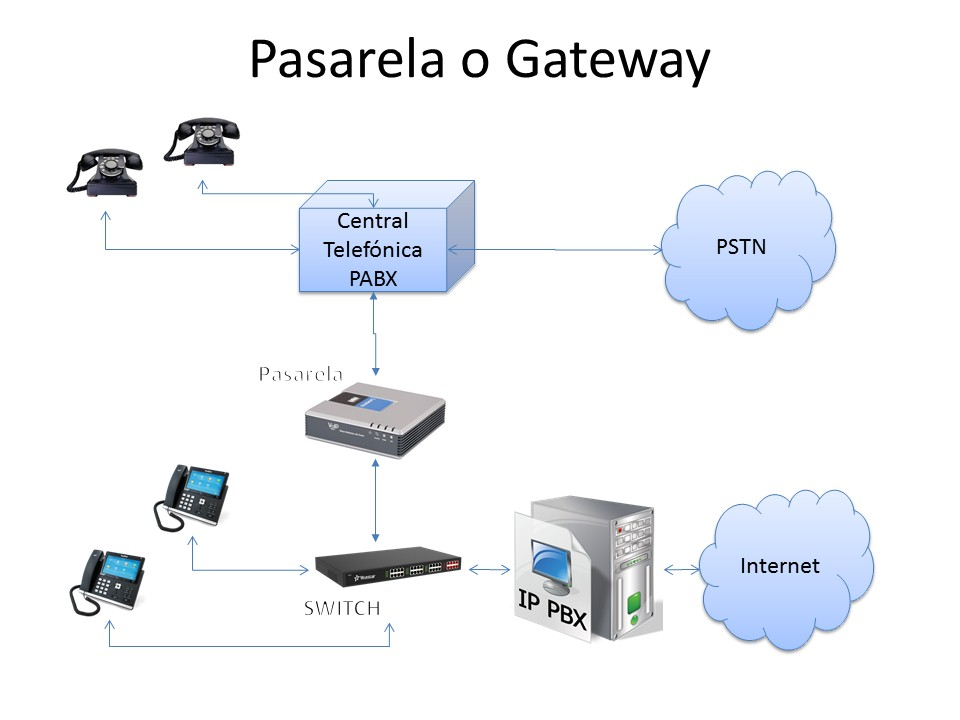
\includegraphics[scale=0.5]{pasarela}
		
		%titulo de la imagen, salen debajo de la imagen y en el indice de imagenes.
		\caption{VoIP combinada con telefonía tradicional a través de una pasarela}
		
		%centrado, por si las moscas
		\centering
		
		%para referencias
		\label{fig:pasarela}
	\end{figure}

Los primeros trabajos sobre digitalización de audio fueron realizados por el Ingeniero Alec Reeves poco antes de la segunda guerra mundial, quien desarrolló un sistema de audio digital con fines militares, sin embargo, la tecnología de comunicaciones de la época todavía no estaba lista para dicho avance. Alec Reeves patento un total de 82\footnote{http://www.quiantium.plus.com/ahr/patents.htm}  inventos entre los que se destaca la idea de Modulacion por impulsos codificados (PCM, Pulse Coded Modulation). Alrededor de los 60s fue que se popularizó la tecnología de PCM pero para entonces ya no eran reclamables los derechos de la patente.

	
		\begin{figure}[h]
			
			%nombre de la imagen, sin extencion. "width=\textwidth" ancho igual al texto
			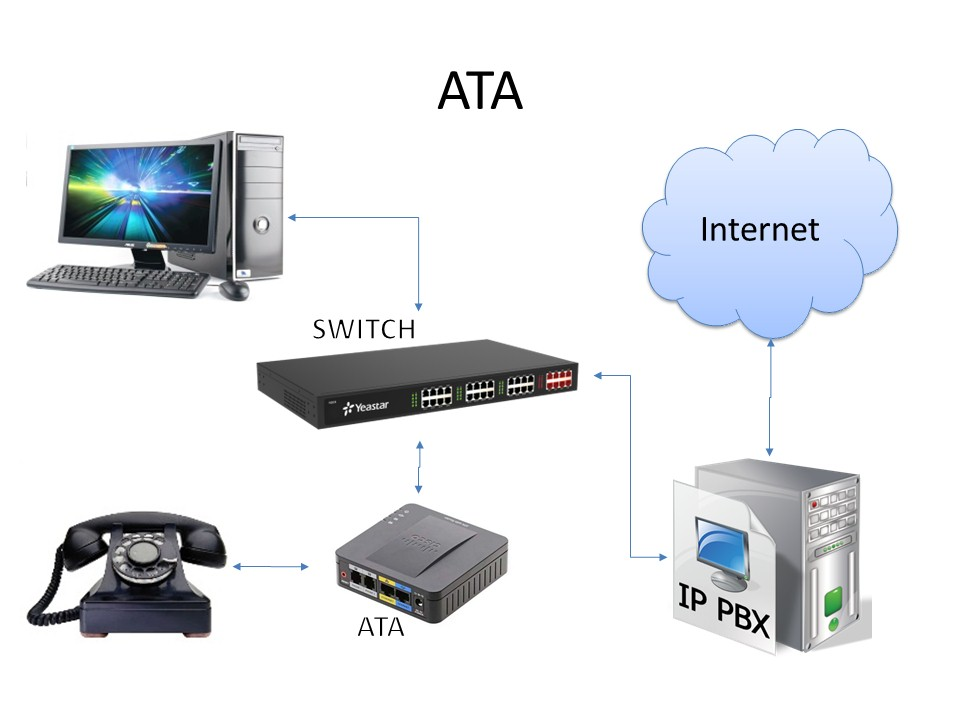
\includegraphics[width=\textwidth]{ata}
			
			%titulo de la imagen, salen debajo de la imagen y en el indice de imagenes.
			\caption{VoIP usando teléfonos analógicos y ATAs}
			
			%centrado, por si las moscas
			\centering
			
			%para referencias
			\label{fig:ata}
		\end{figure}
		
		
Inicialmente la digitalización de voz se basó en codificar la forma de onda de la señal analógica mediante un proceso de muestreo, cuantificación y codificación de la señal, el proceso de PCM. Luego, con el objetivo de reducir la tasa de bits requerida para transmitir la señal, se introdujeron las técnicas predictivas y comenzaron a codificar solo la diferencia entre los valores de las muestras reales y la predicción de la señal en base a la extrapolación de las muestras anteriores.

\subsection{Proceso de digitalización}



\subsection{Códec}

Los códec son algoritmos o dispositivos que realizan la codificación y decodificación de la señal de audio, con usados a menudo en videoconferencias y emisiones de medios de comunicación. La mayoría de los códec provoca pérdidas de información ya que están diseñados para minimizar el tamaño de los datos digitales. Existen códec sin pérdida (lossless) que mantienen la calidad más precisa del sonido, pero generan datos digitales muy grandes que en VoIP no son necesarios.

		\begin{table}[h]
			
			%nombre de la imagen, sin extencion. "width=\textwidth" ancho igual al texto
			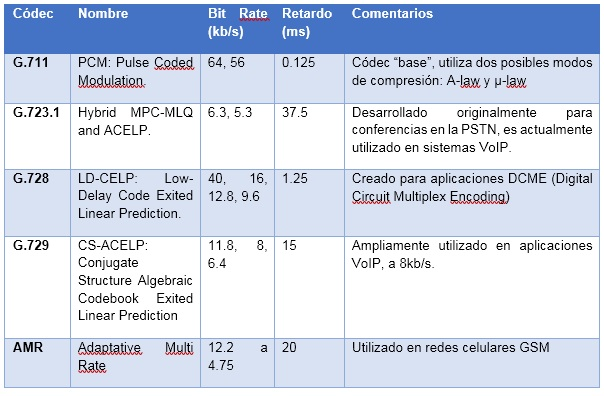
\includegraphics[width=\textwidth]{../tables/codecsnarrowband}
			
			%titulo de la imagen, salen debajo de la imagen y en el indice de imagenes.
			\caption{Códec de banda angosta (Narrowband).}
			
			%centrado, por si las moscas
			\centering
			
			%para referencias
			\label{tab:narrow}
		\end{table}


Existe gran variedad de códecs en el mercado actual y su clasificación puede depender de varios aspectos como la técnica que usan para codificar, el ancho de banda que se muestra o incluso la tasa de bits resultante. En las siguientes tablas se puede apreciar las principales diferencias entre los códec más comunes. En la primera [\ref{tab:narrow}] se pueden apreciar los principales códec de banda angosta, diseñados para digitalizar audio en frecuencias entre 300Hz y 3,4kHz. En la segunda [] se comparan los códec de banda amplia que reproducen señales entre 50Hz y 7kHz. En la tercera [] se encuentran los códec de banda super amplia (frecuencias de 50Hz a 14kHz) y banda completa (frecuencias de 50 Hz a 20 kHz).

AQUI VA LA TABLA DE wideBAND

AQUI VA LA TABLA DE superwideBANDy fullband


\section{Codificación de Video}

	


	%segunda parte
%	\part{Planteamiento del Problema}
%	\part{Propuesta de trabajo}

%blibliografia
%bibliografia, el número indica la cantidad de entradas que tendrá, no puede ser mayor a 99
	\begin{thebibliography}{15}
		\bibitem{switching} 
		T. Eallingford, Switching to VoIP, Beijing: O'Reilly, 2005. .
		
		\bibitem{voiptoip} 
		R. Quispe y G. Suárez.	
		\textit{ Voz sobre IP y Telefonía sobre IP}.
		
		\bibitem{nyquist} 
		H. Nyquist, Certain topics in telegraph transmission theory, de Trans. AIEE, Volumen 47, 1928.
		
		\bibitem{packet}
		B. Hartpence, Packet Guide to Voice over IP, Gravenstein, Sebastopol: O'Reilly Media, Inc, 2013. 
		
		\bibitem{understanding}
		N. Wittenberg, Undertanding Voice over IP Technology, Clifon Park, NY: Delmar Cengage Learning, 2009.
		
		\bibitem{rtp}
		C. Perkings, RTP: Audio and Video for the Internet, Boston: Addison-Wesley, 2003.
		
		\bibitem{undersip}
		A. Jhonston, SIP: Understanding the Session Initiation Protocol, Norwood, Massachusetts: Artech House, 2009.
		
		\bibitem{rfcsip}
		J. Rosenberg, H. Schulzrinne, G. Camarillo, A. Johnston, J. Peterson, R. Sparks, M. Handley y E. Schooler, RFC 3261 SIP: Session Initiation Protocol, 2002. 
		
		\bibitem{siphandbook}
		S. Ilvas y M. Ahson, SIP Handbook, Boca Raton, Florida: CRC Press, 2009.
		
		\bibitem{codif}
		J. Joskowicz, Codificación de Voz y Video, Montevideo, Uruguay: Universidad de la Republica, 2015.
		
	\end{thebibliography}

\end{document}